\documentclass[a4paper,11pt]{ltjsarticle}
\usepackage{luatexja}
\usepackage{amsmath,amssymb,mathtools}
\usepackage{tikz}
\usepackage{tikz-cd}
\usepackage{enumitem}
\usepackage{geometry}
\geometry{margin=25mm}

\usetikzlibrary{arrows.meta,calc,decorations.pathmorphing}

\title{測度論的構造塔と積σ-代数\\\smallskip
{\large--- MeasurableTower モジュールの学部生向け解説 ---}}
\author{CODEX (OpenAI)\\Lean ファイル生成: CODEX (OpenAI)}
\date{2025年11月5日}

\begin{document}

\maketitle

\begin{abstract}
本資料は Lean ファイル \texttt{MyProjects/ST/MeasurableTower.lean} の内容をもとに、
構造塔を測度論的に拡張した \emph{MeasurableTowerWithMin} を学部生向けに解説する。
σ-代数が層として現れる意義、最小層の可測性条件、そして積構造が
標準的な積σ-代数を実現する様子を図式を交えて説明する。
\end{abstract}

\tableofcontents

\section{序論}

ボルバキ的な「集合と構造」の枠組みでは、数学的対象は集合とその上の構造で統一的に扱われる。
`CAT2_complete.lean` で定義された \texttt{StructureTowerWithMin} はこの考え方を体現し、
集合の層が時間の順序に沿って増大する様子を記述していた。

しかし確率論では、層として σ-代数（フィルトレーション）が直接現れる。
`MeasurableTower.lean` では層を \texttt{MeasurableSpace} に置き換えた
`MeasurableTowerWithMin` を導入し、停止時刻の最小性を可測性で捉え直した。

\section{MeasurableTowerWithMin の定義}

\subsection{基本データ}

`MeasurableTowerWithMin` は以下のデータからなる：
\begin{itemize}
  \item 基礎集合 \(X\) と添字集合 \(I\)（半順序付き）
  \item 各添字 \(i \in I\) に対し、σ-代数 \( \mathcal{F}_i \) （Lean では `layer i`）
  \item 単調性 \(i \le j \Rightarrow \mathcal{F}_i \le \mathcal{F}_j\)
  \item 各要素 \(x \in X\) に対し最小添字 \(\mathrm{minLayer}(x)\)
  \item 最小層で単点集合が可測：\(\{x\} \in \mathcal{F}_{\mathrm{minLayer}(x)}\)
  \item 単点集合が可測ならその層は最小層以上：\(\{x\} \in \mathcal{F}_i \Rightarrow \mathrm{minLayer}(x) \le i\)
\end{itemize}

集合塔との違いは、層が単なる集合族ではなく σ-代数そのものになった点にある。
可測性を公理として組み込むことで、停止時刻の直感を Lean 上で直接扱える。

\subsection{図式による概観}

図\ref{fig:tower} は単調性と最小層のイメージを示す。

\begin{figure}[htbp]
  \centering
  \begin{tikzcd}[column sep=huge,row sep=large]
    & \mathcal{F}_{\mathrm{minLayer}(x)} \arrow[dr, hook, "\subseteq"] & \\
    \{x\} \arrow[ur, dashed, "\text{可測}"] \arrow[rr, bend right=20, hook, "\subseteq"] &
      & \mathcal{F}_j
  \end{tikzcd}
  \caption{単点集合が最小層で可測となり、任意の上位層に包含される。}
  \label{fig:tower}
\end{figure}

\section{σ-代数の積と塔の直積}

\subsection{補題 \texorpdfstring{$\mathrm{prod\_le\_prod}$}{prod\_le\_prod}}

Lean 補題 `prod_le_prod` は、σ-代数の包含関係が保たれれば
積σ-代数でも包含が保たれることを示す。
これは `Monotone` 条件の積に対応する重要なステップである。

\subsection{積塔の構成}

`MeasurableTowerWithMin.prod` では、基礎集合と添字集合を直積にし、
層を `MeasurableSpace.prod` で定義する。
単点集合の可測性は図\ref{fig:prod}のように直積集合の可測性から得られる。

\begin{figure}[htbp]
  \centering
  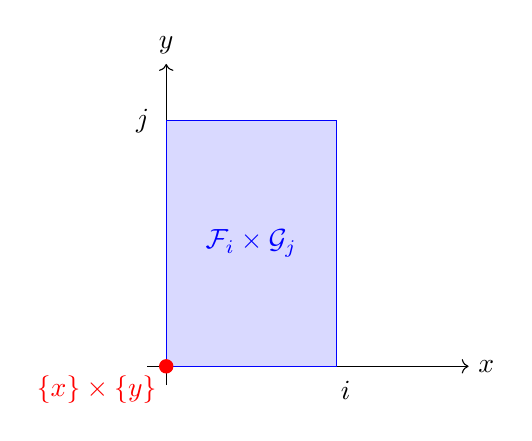
\begin{tikzpicture}[scale=1.2]
    \draw[->] (-0.2,0) -- (3.2,0) node[right] {$x$};
    \draw[->] (0,-0.2) -- (0,3.2) node[above] {$y$};
    \draw[fill=blue!15, draw=blue] (0,0) rectangle (1.8,2.6);
    \draw[dashed, blue] (0,2.6) -- (1.8,2.6);
    \draw[dashed, blue] (1.8,0) -- (1.8,2.6);
    \node[blue] at (0.9,1.3) {$\mathcal{F}_{i} \times \mathcal{G}_{j}$};
    \node at (1.9,-0.25) {$i$};
    \node at (-0.25,2.6) {$j$};
    \filldraw[red] (0,0) circle (2pt) node[below left] {$\{x\} \times \{y\}$};
  \end{tikzpicture}
  \caption{単点集合の直積は積σ-代数で可測（`singleton\_prod\_singleton`）。}
  \label{fig:prod}
\end{figure}

Lean では `MeasurableSet.prod` と `singleton_prod_singleton` を用いて
単点集合が積σ-代数で可測であることを示し、
最小層の最小性を `measurableSet_prod_of_nonempty` で分解して証明する。

\section{例：自明な測度塔}

`trivialMeasurableTowerNat` は各層が最大σ-代数（すべての集合が可測）である簡単な例である。
ここでは最小層は常に 0 となり、自己直積でも
\[
  \mathrm{minLayer}((0,0)) = (0,0)
\]
が即座に得られる。

\section{StructureTower からの関手生成の考察}

集合塔から σ-代数塔へ写す `GenerateSigmaAlgebra` を考えるなら、
各層を `MeasurableSpace.generateFrom` で σ-代数に昇格させるのが自然である。
ただし最小層の条件を保つには、単点集合が生成元に含まれる等の追加仮定が必要である。
この視点は「集合論的な生成系の積」と「σ-代数の積」が一致しないことを明瞭に示す。

\section{まとめと今後の展望}

\begin{itemize}
  \item 層を σ-代数に置き換えることで、停止時刻の最小性を可測性で表現できた。
  \item 積構造では `MeasurableSpace.prod` が自然に現れ、標準的な積σ-代数を再現した。
  \item 集合塔から σ-代数塔への関手構成には、単点集合の扱いなど追加条件が必要である。
\end{itemize}

今後は、停止時刻の射（`Hom`）を測度論版にも拡張し、
既存の確率論ファイルと接続することで、より実践的なフィルトレーションの理論を
Lean 上で構築できるだろう。

\end{document}
